% ============================================================
% 讲义 — 人教版高三选择性必修第三册 第7章 随机变量及其分布
% 编译命令：xelatex -interaction=nonstopmode 文件名.tex
% ============================================================
\documentclass[12pt, a4paper]{ctexart}
\usepackage[margin=2.2cm]{geometry}
\usepackage{amsmath, amssymb}
\usepackage{enumitem}
\usepackage{tcolorbox}
\usepackage{booktabs}
\usepackage{array}
\usepackage{fancyhdr}
\usepackage{xcolor}
\usepackage{tikz}
\usepackage{hyperref}
\usepackage{graphicx}
\usepackage{multirow}
\usepackage{pgfplots}
\pgfplotsset{compat=1.18}

% 颜色定义
\definecolor{mainblue}{RGB}{41, 98, 168}
\definecolor{lightblue}{RGB}{230, 240, 255}
\definecolor{tipgreen}{RGB}{34, 139, 87}
\definecolor{lightgreen}{RGB}{235, 250, 240}
\definecolor{warnred}{RGB}{200, 50, 50}
\definecolor{lightred}{RGB}{255, 240, 240}
\definecolor{examorange}{RGB}{210, 120, 20}
\definecolor{lightorange}{RGB}{255, 248, 235}
\definecolor{apppurple}{RGB}{120, 60, 170}
\definecolor{lightpurple}{RGB}{245, 238, 255}

% 页眉页脚
\pagestyle{fancy}
\fancyhf{}
\fancyhead[L]{\small\textcolor{mainblue}{\textbf{人教版高三选必3 · 第7章 随机变量及其分布}}}
\fancyhead[R]{\small\textcolor{mainblue}{随机变量及其分布讲义}}
\fancyfoot[C]{\small —\ \thepage\ —}
\renewcommand{\headrulewidth}{0.6pt}
\renewcommand{\headrule}{\hbox to\headwidth{\color{mainblue}\leaders\hrule height \headrulewidth\hfill}}
\renewcommand{\footrulewidth}{0pt}

% tcolorbox 样式
\newtcolorbox{knowledgebox}[1][]{%
  colback=lightblue, colframe=mainblue,
  fonttitle=\bfseries\large, title=#1,
  arc=3mm, boxrule=0.8pt,
  left=8pt, right=8pt, top=6pt, bottom=6pt
}

\newtcolorbox{tipbox}[1][]{%
  colback=lightgreen, colframe=tipgreen,
  fonttitle=\bfseries, title=#1,
  arc=2mm, boxrule=0.6pt,
  left=6pt, right=6pt, top=4pt, bottom=4pt
}

\newtcolorbox{warnbox}[1][]{%
  colback=lightred, colframe=warnred,
  fonttitle=\bfseries, title=#1,
  arc=2mm, boxrule=0.6pt,
  left=6pt, right=6pt, top=4pt, bottom=4pt
}

\newtcolorbox{examplebox}[1][]{%
  colback=lightorange, colframe=examorange,
  fonttitle=\bfseries, title=#1,
  arc=3mm, boxrule=0.8pt,
  left=8pt, right=8pt, top=6pt, bottom=6pt
}

\newtcolorbox{appbox}[1][]{%
  colback=lightpurple, colframe=apppurple,
  fonttitle=\bfseries, title=#1,
  arc=3mm, boxrule=0.8pt,
  left=8pt, right=8pt, top=6pt, bottom=6pt
}

\setCJKmainfont{Hiragino Sans GB}
\setCJKsansfont{Heiti SC}

\begin{document}

% ============ 标题页 ============
\begin{center}
{\Huge\bfseries\textcolor{mainblue}{第7章\quad 随机变量及其分布}}\\[12pt]
{\Large\textcolor{gray}{讲\quad 义}}\\[8pt]
\rule{0.6\textwidth}{1pt}\\[8pt]
{\normalsize 适用：人教版\quad 高三选择性必修第三册\quad |\quad 课时：4课时}
\end{center}
\vspace{10pt}

% ============================================================
%  第一部分：知识点讲解
% ============================================================
\section*{\textcolor{mainblue}{一、知识点讲解}}

% ------ 7.1 离散型随机变量 ------
\subsection*{7.1\quad 离散型随机变量}

\begin{knowledgebox}[离散型随机变量的定义]
在随机试验中，我们确定一个对应关系，使得每一个试验结果都用一个\textbf{确定的数}来表示，这个对应关系就是一个\textbf{随机变量}，通常用大写字母 $X, Y, Z, \ldots$ 表示。

如果随机变量 $X$ 的所有可能取值为\textbf{有限个}或可以\textbf{一一列举}的无限多个，则称 $X$ 为\textbf{离散型随机变量}。
\end{knowledgebox}

\begin{tipbox}[判断随机变量是否离散的方法]
\begin{enumerate}[label=(\arabic*)]
  \item 列出随机变量所有可能的取值；
  \item 若取值为有限个或可列无限个，则为离散型随机变量；
  \item 若取值为某区间上的连续值（如身高、体重），则为连续型随机变量。
\end{enumerate}
\end{tipbox}

% ------ 7.2 离散型随机变量的分布列 ------
\subsection*{7.2\quad 离散型随机变量的分布列}

\begin{knowledgebox}[分布列的定义与性质]
设离散型随机变量 $X$ 的所有可能取值为 $x_1, x_2, \ldots, x_n$，且
\[
P(X = x_i) = p_i \quad (i = 1, 2, \ldots, n)
\]
则称下表为 $X$ 的\textbf{概率分布列}（简称\textbf{分布列}）：
\[
\begin{array}{c|cccc}
X & x_1 & x_2 & \cdots & x_n \\
\hline
P & p_1 & p_2 & \cdots & p_n
\end{array}
\]
分布列满足以下性质：
\begin{enumerate}[label=(\arabic*)]
  \item $p_i \geqslant 0$，$i = 1, 2, \ldots, n$（\textbf{非负性}）；
  \item $p_1 + p_2 + \cdots + p_n = 1$（\textbf{归一性}）。
\end{enumerate}
\end{knowledgebox}

% ------ 7.3 离散型随机变量的期望与方差 ------
\subsection*{7.3\quad 离散型随机变量的期望与方差}

\begin{knowledgebox}[数学期望]
若离散型随机变量 $X$ 的分布列为 $P(X = x_i) = p_i$，$i = 1, 2, \ldots, n$，则称
\[
E(X) = x_1 p_1 + x_2 p_2 + \cdots + x_n p_n = \sum_{i=1}^{n} x_i p_i
\]
为 $X$ 的\textbf{数学期望}（或\textbf{均值}）。

期望的性质：
\begin{enumerate}[label=(\arabic*)]
  \item $E(c) = c$（$c$ 为常数）；
  \item $E(aX + b) = aE(X) + b$（线性性质）；
  \item $E(X_1 + X_2) = E(X_1) + E(X_2)$。
\end{enumerate}
\end{knowledgebox}

\begin{knowledgebox}[方差与标准差]
\[
D(X) = \sum_{i=1}^{n} [x_i - E(X)]^2 \cdot p_i = E(X^2) - [E(X)]^2
\]
称 $D(X)$ 为 $X$ 的\textbf{方差}，$\sqrt{D(X)}$ 为 $X$ 的\textbf{标准差}。

方差的性质：
\begin{enumerate}[label=(\arabic*)]
  \item $D(c) = 0$；
  \item $D(aX + b) = a^2 D(X)$；
  \item 若 $X_1, X_2$ 相互独立，则 $D(X_1 + X_2) = D(X_1) + D(X_2)$。
\end{enumerate}
\end{knowledgebox}

\begin{warnbox}[易错提醒]
\begin{itemize}
  \item $D(aX + b) = a^2 D(X)$，常数 $b$ 不影响方差，系数 $a$ 需要\textbf{平方}；
  \item 计算方差时，用公式 $D(X) = E(X^2) - [E(X)]^2$ 往往比定义式更简便；
  \item 方差反映的是随机变量取值的\textbf{离散程度}，而非均值大小。
\end{itemize}
\end{warnbox}

% ------ 7.4 二项分布 ------
\subsection*{7.4\quad 二项分布}

\begin{knowledgebox}[伯努利试验与二项分布]
如果一次试验只有两个结果（"成功"或"失败"），将该试验独立重复地进行 $n$ 次，则称为\textbf{$n$ 重伯努利试验}。

在 $n$ 重伯努利试验中，设每次试验"成功"的概率为 $p$（$0 < p < 1$），记 $X$ 为 $n$ 次试验中"成功"的次数，则
\[
P(X = k) = \mathrm{C}_n^k \, p^k (1-p)^{n-k}, \quad k = 0, 1, 2, \ldots, n
\]
此时称 $X$ 服从\textbf{二项分布}，记为 $X \sim B(n, p)$。

\medskip
期望与方差：
\[
E(X) = np, \qquad D(X) = np(1-p)
\]
\end{knowledgebox}

\begin{tipbox}[二项分布的识别要点]
\begin{enumerate}[label=(\arabic*)]
  \item 每次试验只有两个结果；
  \item 每次试验中"成功"的概率不变；
  \item 各次试验相互独立；
  \item 共进行 $n$ 次试验。
\end{enumerate}
同时满足以上四个条件，才可使用二项分布模型。
\end{tipbox}

% ------ 7.5 超几何分布 ------
\subsection*{7.5\quad 超几何分布}

\begin{knowledgebox}[超几何分布]
设 $N$ 件产品中有 $M$ 件次品，从中不放回地抽取 $n$ 件，记 $X$ 为抽取到的次品数，则
\[
P(X = k) = \frac{\mathrm{C}_M^k \, \mathrm{C}_{N-M}^{n-k}}{\mathrm{C}_N^n}, \quad k = 0, 1, 2, \ldots, \min(M, n)
\]
称 $X$ 服从\textbf{超几何分布}。

\medskip
期望与方差：
\[
E(X) = \frac{nM}{N}, \qquad D(X) = \frac{nM(N-M)(N-n)}{N^2(N-1)}
\]
\end{knowledgebox}

\begin{warnbox}[二项分布与超几何分布的区别]
\begin{itemize}
  \item \textbf{二项分布}：有放回抽样（或独立重复试验），每次试验概率不变；
  \item \textbf{超几何分布}：不放回抽样，每次抽取后总体结构改变；
  \item 当 $N$ 很大而 $n$ 相对较小时，超几何分布可近似为二项分布。
\end{itemize}
\end{warnbox}

% ------ 7.6 正态分布 ------
\subsection*{7.6\quad 正态分布}

\begin{knowledgebox}[正态分布]
如果连续型随机变量 $X$ 的概率密度函数为
\[
f(x) = \frac{1}{\sigma\sqrt{2\pi}} \, e^{-\frac{(x - \mu)^2}{2\sigma^2}}, \quad x \in (-\infty, +\infty)
\]
其中 $\mu$ 为均值，$\sigma > 0$ 为标准差，则称 $X$ 服从\textbf{正态分布}，记为 $X \sim N(\mu, \sigma^2)$。

特别地，当 $\mu = 0$，$\sigma = 1$ 时，称 $X$ 服从\textbf{标准正态分布}，记为 $X \sim N(0, 1)$。
\end{knowledgebox}

\begin{knowledgebox}[正态分布的性质]
\begin{enumerate}[label=(\arabic*)]
  \item 密度曲线关于 $x = \mu$ \textbf{对称}；
  \item $x = \mu$ 时 $f(x)$ 取最大值 $\dfrac{1}{\sigma\sqrt{2\pi}}$；
  \item $\sigma$ 越小，曲线越"瘦高"（取值越集中于 $\mu$）；$\sigma$ 越大，曲线越"矮胖"（取值越分散）；
  \item $E(X) = \mu$，$D(X) = \sigma^2$。
\end{enumerate}
\end{knowledgebox}

\begin{knowledgebox}[$3\sigma$ 准则]
若 $X \sim N(\mu, \sigma^2)$，则
\begin{align*}
P(\mu - \sigma < X < \mu + \sigma) &\approx 0.6827, \\
P(\mu - 2\sigma < X < \mu + 2\sigma) &\approx 0.9545, \\
P(\mu - 3\sigma < X < \mu + 3\sigma) &\approx 0.9973.
\end{align*}
这就是正态分布的\textbf{$3\sigma$ 准则}（也称"68-95-99.7 法则"）。
\end{knowledgebox}

% 正态分布密度函数图像
\begin{center}
\begin{tikzpicture}
\begin{axis}[
  width=12cm, height=6cm,
  xlabel={$x$}, ylabel={$f(x)$},
  domain=-4:4, samples=100,
  axis lines=middle,
  xmin=-4.5, xmax=4.5, ymin=0, ymax=0.45,
  xtick={-3,-2,-1,0,1,2,3},
  xticklabels={$\mu{-}3\sigma$,$\mu{-}2\sigma$,$\mu{-}\sigma$,$\mu$,$\mu{+}\sigma$,$\mu{+}2\sigma$,$\mu{+}3\sigma$},
  ytick=\empty,
  legend style={at={(0.98,0.98)}, anchor=north east},
  every axis plot/.append style={thick}
]
\addplot[mainblue, fill=lightblue, fill opacity=0.3] {exp(-x^2/2)/sqrt(2*pi)};
\addlegendentry{$\sigma$ 较小}
\addplot[warnred, dashed, fill=lightred, fill opacity=0.2] {exp(-x^2/(2*2.25))/(sqrt(2*pi)*1.5)};
\addlegendentry{$\sigma$ 较大}
\end{axis}
\end{tikzpicture}
\end{center}

\vspace{6pt}

\begin{warnbox}[易错提醒]
\begin{itemize}
  \item 正态分布中 $P(X = a) = 0$，因此 $P(a < X < b) = P(a \leqslant X \leqslant b)$；
  \item 利用对称性：$P(X < \mu - a) = P(X > \mu + a)$；
  \item 标准化公式：若 $X \sim N(\mu, \sigma^2)$，则 $Z = \dfrac{X - \mu}{\sigma} \sim N(0, 1)$。
\end{itemize}
\end{warnbox}

% ============================================================
%  第二部分：例题精讲
% ============================================================
\section*{\textcolor{examorange}{二、例题精讲}}

% --- 例1 ---
\begin{examplebox}[【例1】求分布列并计算期望方差]
一个袋中有 $5$ 个白球和 $3$ 个黑球，从中任取 $3$ 个球。设 $X$ 为取到黑球的个数，求 $X$ 的分布列、期望和方差。
\end{examplebox}

\textbf{解}：$X$ 的可能取值为 $0, 1, 2, 3$。

由超几何分布：
\begin{align*}
P(X=0) &= \frac{\mathrm{C}_3^0 \mathrm{C}_5^3}{\mathrm{C}_8^3} = \frac{10}{56} = \frac{5}{28} \\[4pt]
P(X=1) &= \frac{\mathrm{C}_3^1 \mathrm{C}_5^2}{\mathrm{C}_8^3} = \frac{30}{56} = \frac{15}{28} \\[4pt]
P(X=2) &= \frac{\mathrm{C}_3^2 \mathrm{C}_5^1}{\mathrm{C}_8^3} = \frac{15}{56} \\[4pt]
P(X=3) &= \frac{\mathrm{C}_3^3 \mathrm{C}_5^0}{\mathrm{C}_8^3} = \frac{1}{56}
\end{align*}

分布列为：
\[
\begin{array}{c|cccc}
X & 0 & 1 & 2 & 3 \\
\hline
P & \dfrac{5}{28} & \dfrac{15}{28} & \dfrac{15}{56} & \dfrac{1}{56}
\end{array}
\]

验证归一性：$\dfrac{5}{28} + \dfrac{15}{28} + \dfrac{15}{56} + \dfrac{1}{56} = \dfrac{10+30+15+1}{56} = 1$。\checkmark

\begin{align*}
E(X) &= 0 \times \frac{5}{28} + 1 \times \frac{15}{28} + 2 \times \frac{15}{56} + 3 \times \frac{1}{56}
= \frac{0 + 30 + 30 + 3}{56} = \frac{63}{56} = \frac{9}{8} = 1.125
\end{align*}

也可以用超几何分布期望公式验证：$E(X) = \dfrac{nM}{N} = \dfrac{3 \times 3}{8} = \dfrac{9}{8}$。\checkmark

\begin{align*}
E(X^2) &= 0 + 1 \times \frac{15}{28} + 4 \times \frac{15}{56} + 9 \times \frac{1}{56}
= \frac{30 + 60 + 9}{56} = \frac{99}{56}
\end{align*}

\[
D(X) = E(X^2) - [E(X)]^2 = \frac{99}{56} - \frac{81}{64} = \frac{99 \times 8 - 81 \times 7}{448} = \frac{792 - 567}{448} = \frac{225}{448} \approx 0.502
\]

\begin{tipbox}[方法总结]
超几何分布的分布列计算用组合数公式，期望和方差可直接用公式验证，减少计算量。
\end{tipbox}

% --- 例2 ---
\begin{examplebox}[【例2】二项分布的概率计算]
某射手每次射击命中目标的概率为 $0.8$，独立射击 $5$ 次。求：(1) 恰好命中 $3$ 次的概率；(2) 至少命中 $4$ 次的概率。
\end{examplebox}

\textbf{解}：设 $X$ 为命中的次数，则 $X \sim B(5, 0.8)$。

(1) 恰好命中3次：
\[
P(X=3) = \mathrm{C}_5^3 \times 0.8^3 \times 0.2^2 = 10 \times 0.512 \times 0.04 = 0.2048
\]

(2) 至少命中4次：
\begin{align*}
P(X \geqslant 4) &= P(X=4) + P(X=5) \\
&= \mathrm{C}_5^4 \times 0.8^4 \times 0.2 + \mathrm{C}_5^5 \times 0.8^5 \\
&= 5 \times 0.4096 \times 0.2 + 0.32768 \\
&= 0.4096 + 0.32768 = 0.73728
\end{align*}

% --- 例3 ---
\begin{examplebox}[【例3】分布列的性质应用]
设随机变量 $X$ 的分布列为 $P(X = k) = \dfrac{c}{k(k+1)}$，$k = 1, 2, 3, 4$。求常数 $c$ 的值及 $E(X)$。
\end{examplebox}

\textbf{解}：由归一性 $\displaystyle\sum_{k=1}^{4} P(X=k) = 1$：
\begin{align*}
\sum_{k=1}^{4} \frac{c}{k(k+1)} &= c\sum_{k=1}^{4}\left(\frac{1}{k} - \frac{1}{k+1}\right) \\
&= c\left[\left(\frac{1}{1} - \frac{1}{2}\right) + \left(\frac{1}{2} - \frac{1}{3}\right) + \left(\frac{1}{3} - \frac{1}{4}\right) + \left(\frac{1}{4} - \frac{1}{5}\right)\right] \\
&= c\left(1 - \frac{1}{5}\right) = \frac{4c}{5} = 1
\end{align*}
所以 $c = \dfrac{5}{4}$。

各概率为：
\[
P(X=1) = \frac{5}{8},\quad P(X=2) = \frac{5}{24},\quad P(X=3) = \frac{5}{48},\quad P(X=4) = \frac{5}{80} = \frac{1}{16}
\]

\[
E(X) = 1 \times \frac{5}{8} + 2 \times \frac{5}{24} + 3 \times \frac{5}{48} + 4 \times \frac{1}{16}
= \frac{5}{8} + \frac{5}{12} + \frac{5}{16} + \frac{1}{4}
= \frac{30 + 20 + 15 + 12}{48} = \frac{77}{48}
\]

\begin{tipbox}[方法总结]
裂项求和在求分布列中的常数时非常常用：$\dfrac{1}{k(k+1)} = \dfrac{1}{k} - \dfrac{1}{k+1}$。
\end{tipbox}

% --- 例4 ---
\begin{examplebox}[【例4】正态分布的区间概率]
已知 $X \sim N(100, 25)$，求 $P(95 < X < 105)$ 与 $P(X > 110)$。
\end{examplebox}

\textbf{解}：$\mu = 100$，$\sigma = 5$。

(1) $P(95 < X < 105) = P(\mu - \sigma < X < \mu + \sigma) \approx 0.6827$。

(2) $P(X > 110)$：由于 $110 = \mu + 2\sigma$，利用对称性：
\[
P(X > \mu + 2\sigma) = \frac{1 - P(\mu - 2\sigma < X < \mu + 2\sigma)}{2} = \frac{1 - 0.9545}{2} = 0.02275
\]

% --- 例5 ---
\begin{examplebox}[【例5】二项分布的期望方差及图像]
设 $X \sim B(6, 0.3)$，求 $E(X)$，$D(X)$，并画出分布列的柱状图。
\end{examplebox}

\textbf{解}：
\[
E(X) = np = 6 \times 0.3 = 1.8
\]
\[
D(X) = np(1-p) = 6 \times 0.3 \times 0.7 = 1.26
\]

各取值概率：
\begin{align*}
P(X=0) &= 0.7^6 \approx 0.1176 \\
P(X=1) &= \mathrm{C}_6^1 \times 0.3 \times 0.7^5 \approx 0.3025 \\
P(X=2) &= \mathrm{C}_6^2 \times 0.3^2 \times 0.7^4 \approx 0.3241 \\
P(X=3) &= \mathrm{C}_6^3 \times 0.3^3 \times 0.7^3 \approx 0.1852 \\
P(X=4) &= \mathrm{C}_6^4 \times 0.3^4 \times 0.7^2 \approx 0.0595 \\
P(X=5) &= \mathrm{C}_6^5 \times 0.3^5 \times 0.7 \approx 0.0102 \\
P(X=6) &= 0.3^6 \approx 0.0007
\end{align*}

\begin{center}
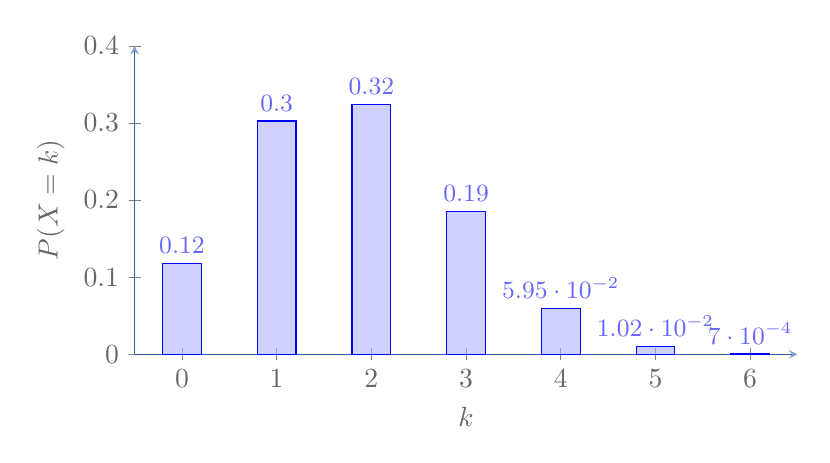
\begin{tikzpicture}
\begin{axis}[
  ybar, bar width=14pt,
  width=10cm, height=5.5cm,
  xlabel={$k$}, ylabel={$P(X=k)$},
  xmin=-0.5, xmax=6.5, ymin=0, ymax=0.4,
  xtick={0,1,2,3,4,5,6},
  nodes near coords,
  every node near coord/.append style={font=\small},
  enlarge x limits=0.12,
  axis lines=left,
  fill=mainblue, draw=mainblue,
  fill opacity=0.6
]
\addplot coordinates {
  (0, 0.1176)
  (1, 0.3025)
  (2, 0.3241)
  (3, 0.1852)
  (4, 0.0595)
  (5, 0.0102)
  (6, 0.0007)
};
\end{axis}
\end{tikzpicture}
\end{center}

% --- 例6 ---
\begin{examplebox}[【例6】正态分布标准化与概率计算]
某次考试成绩 $X \sim N(75, 100)$（即 $\mu=75$，$\sigma=10$）。若规定成绩在 $85$ 分以上为优秀，求优秀的概率。
\end{examplebox}

\textbf{解}：$P(X > 85)$。

标准化：令 $Z = \dfrac{X - 75}{10}$，则 $Z \sim N(0, 1)$。

\[
P(X > 85) = P\left(Z > \frac{85 - 75}{10}\right) = P(Z > 1)
\]

由标准正态分布的对称性：
\[
P(Z > 1) = \frac{1 - P(-1 < Z < 1)}{2} = \frac{1 - 0.6827}{2} \approx 0.1587
\]

所以优秀的概率约为 $15.87\%$。

% --- 例7 ---
\begin{examplebox}[【例7】综合应用：产品检验]
一批产品共 $100$ 件，其中 $5$ 件次品。采用两种方案检验：\\
方案甲：从中任取 $10$ 件检验，$X$ 为次品数；\\
方案乙：逐件有放回地抽取检验，取 $10$ 件，$Y$ 为次品数。\\
分别求 $E(X)$ 和 $E(Y)$，并比较两方案。
\end{examplebox}

\textbf{解}：

方案甲（不放回）：$X$ 服从超几何分布，$N=100$，$M=5$，$n=10$。
\[
E(X) = \frac{nM}{N} = \frac{10 \times 5}{100} = 0.5
\]

方案乙（有放回）：每次抽到次品的概率 $p = \dfrac{5}{100} = 0.05$，$Y \sim B(10, 0.05)$。
\[
E(Y) = np = 10 \times 0.05 = 0.5
\]

两种方案的期望相同，均为 $0.5$。

但方差不同：
\[
D(X) = \frac{10 \times 5 \times 95 \times 90}{100^2 \times 99} = \frac{427500}{990000} \approx 0.4318
\]
\[
D(Y) = 10 \times 0.05 \times 0.95 = 0.475
\]

$D(X) < D(Y)$，说明不放回抽样方案（甲）的检测结果更稳定。

\begin{tipbox}[方法总结]
当总体容量 $N$ 很大而抽样量 $n$ 较小时，超几何分布与二项分布的差异很小，可用二项分布近似。
\end{tipbox}

% --- 例8 ---
\begin{examplebox}[【例8】二项分布与超几何分布辨析]
一个盒中有 $8$ 个红球和 $4$ 个白球。(1) 有放回地取 $3$ 次，每次取 $1$ 个，求恰好 $2$ 次取到红球的概率；(2) 不放回地取 $3$ 个，求恰好 $2$ 个红球的概率。
\end{examplebox}

\textbf{解}：

(1) 有放回：每次取到红球的概率 $p = \dfrac{8}{12} = \dfrac{2}{3}$，设 $X$ 为红球次数，$X \sim B\!\left(3, \dfrac{2}{3}\right)$。
\[
P(X=2) = \mathrm{C}_3^2 \left(\frac{2}{3}\right)^2 \left(\frac{1}{3}\right)^1 = 3 \times \frac{4}{9} \times \frac{1}{3} = \frac{4}{9}
\]

(2) 不放回：$N=12$，$M=8$，$n=3$，设 $Y$ 为红球数。
\[
P(Y=2) = \frac{\mathrm{C}_8^2 \mathrm{C}_4^1}{\mathrm{C}_{12}^3} = \frac{28 \times 4}{220} = \frac{112}{220} = \frac{28}{55}
\]

两者概率不同：$\dfrac{4}{9} \approx 0.444$ vs $\dfrac{28}{55} \approx 0.509$。

\begin{warnbox}[辨析要点]
有放回是二项分布，不放回是超几何分布。两者模型不同，结果通常不相等。
\end{warnbox}

% ============================================================
%  第三部分：应用题
% ============================================================
\section*{\textcolor{apppurple}{三、应用题}}

% --- 应用1 ---
\begin{appbox}[【应用1】保险精算]
某保险公司有 $10000$ 人投保，每人每年交保费 $200$ 元。根据统计，每人一年内出险的概率为 $0.002$，出险后保险公司赔付 $50000$ 元。设 $X$ 为一年内出险的人数。
\begin{enumerate}[label=(\arabic*)]
  \item 求 $X$ 的分布列（写出分布名称即可）；
  \item 求 $E(X)$ 及保险公司一年的期望利润。
\end{enumerate}
\end{appbox}

\textbf{解}：

(1) 每人出险相互独立，概率 $p = 0.002$，$n = 10000$。
$X \sim B(10000, 0.002)$。

(2) $E(X) = np = 10000 \times 0.002 = 20$ 人。

保险公司一年的保费收入：$10000 \times 200 = 2000000$ 元。

期望赔付：$E(X) \times 50000 = 20 \times 50000 = 1000000$ 元。

期望利润：$2000000 - 1000000 = 1000000$ 元 $= 100$ 万元。

% --- 应用2 ---
\begin{appbox}[【应用2】质量控制]
某工厂生产的灯泡寿命 $X$（单位：小时）服从正态分布 $X \sim N(1000, 2500)$。
\begin{enumerate}[label=(\arabic*)]
  \item 求灯泡寿命在 $950$ 至 $1050$ 小时之间的概率；
  \item 若工厂规定寿命低于 $900$ 小时的灯泡为不合格品，求不合格品率；
  \item 在 $1000$ 个灯泡中，预计有多少个寿命超过 $1050$ 小时？
\end{enumerate}
\end{appbox}

\textbf{解}：$\mu = 1000$，$\sigma = \sqrt{2500} = 50$。

(1) $950 = \mu - \sigma$，$1050 = \mu + \sigma$。
\[
P(950 < X < 1050) = P(\mu - \sigma < X < \mu + \sigma) \approx 0.6827
\]

(2) $900 = \mu - 2\sigma$。
\[
P(X < 900) = P(X < \mu - 2\sigma) = \frac{1 - P(\mu - 2\sigma < X < \mu + 2\sigma)}{2} = \frac{1 - 0.9545}{2} = 0.02275
\]
不合格品率约为 $2.28\%$。

(3) $P(X > 1050) = P(X > \mu + \sigma) = \dfrac{1 - 0.6827}{2} = 0.15865$。

预计寿命超过 $1050$ 小时的灯泡数：$1000 \times 0.15865 \approx 159$ 个。

% --- 应用3 ---
\begin{appbox}[【应用3】抽奖活动设计]
某商场设计抽奖活动：箱中有 $20$ 个球，其中 $4$ 个红球，$16$ 个白球。顾客从中不放回地摸 $3$ 个球。规则如下：
\begin{itemize}
  \item 摸到 $3$ 个红球：一等奖，奖金 $500$ 元；
  \item 摸到恰好 $2$ 个红球：二等奖，奖金 $100$ 元；
  \item 摸到恰好 $1$ 个红球：三等奖，奖金 $10$ 元；
  \item 摸到 $0$ 个红球：不中奖。
\end{itemize}
\begin{enumerate}[label=(\arabic*)]
  \item 求各奖项的概率；
  \item 求顾客获得奖金的期望值；若每人参与需交 $15$ 元，商场是否有盈利空间？
\end{enumerate}
\end{appbox}

\textbf{解}：$N=20$，$M=4$，$n=3$，$X$ 为红球数。

(1) 各概率：
\begin{align*}
P(X=3) &= \frac{\mathrm{C}_4^3}{\mathrm{C}_{20}^3} = \frac{4}{1140} = \frac{1}{285} \approx 0.00351 \\[4pt]
P(X=2) &= \frac{\mathrm{C}_4^2 \mathrm{C}_{16}^1}{\mathrm{C}_{20}^3} = \frac{6 \times 16}{1140} = \frac{96}{1140} = \frac{8}{95} \approx 0.08421 \\[4pt]
P(X=1) &= \frac{\mathrm{C}_4^1 \mathrm{C}_{16}^2}{\mathrm{C}_{20}^3} = \frac{4 \times 120}{1140} = \frac{480}{1140} = \frac{8}{19} \approx 0.42105 \\[4pt]
P(X=0) &= \frac{\mathrm{C}_{16}^3}{\mathrm{C}_{20}^3} = \frac{560}{1140} = \frac{28}{57} \approx 0.49123
\end{align*}

验证：$\dfrac{1}{285} + \dfrac{8}{95} + \dfrac{8}{19} + \dfrac{28}{57} = \dfrac{1 + 24 + 120 + 140}{285} = \dfrac{285}{285} = 1$。\checkmark

(2) 期望奖金：
\begin{align*}
E(\text{奖金}) &= 500 \times \frac{1}{285} + 100 \times \frac{8}{95} + 10 \times \frac{8}{19} + 0 \\
&= \frac{500}{285} + \frac{800}{95} + \frac{80}{19} \\
&= \frac{500}{285} + \frac{2400}{285} + \frac{1200}{285} = \frac{4100}{285} \approx 14.39 \text{ 元}
\end{align*}

每人交 $15$ 元，期望支出约 $14.39$ 元，商场每人期望盈利约 $0.61$ 元。有微薄的盈利空间。

% ============================================================
%  第四部分：课堂练习
% ============================================================
\section*{\textcolor{tipgreen}{四、课堂练习}}

\begin{enumerate}
  \item 设随机变量 $X$ 的分布列为
  \[
  \begin{array}{c|ccc}
  X & -1 & 0 & 1 \\
  \hline
  P & a & 0.3 & 0.4
  \end{array}
  \]
  求 $a$ 的值，$E(X)$ 和 $D(X)$。

  \item 已知 $X \sim B(8, 0.5)$，求 $P(X = 4)$ 和 $P(X \geqslant 6)$。

  \item 一批零件共 $50$ 个，其中 $4$ 个是次品。从中不放回地取 $5$ 个，设 $X$ 为次品数，求 $P(X \leqslant 1)$。

  \item 某地区考生高考数学成绩服从正态分布 $N(90, 225)$。
  \begin{enumerate}[label=(\arabic*)]
    \item 求成绩在 $75$ 至 $105$ 之间的概率；
    \item 若录取分数线为 $120$ 分，求被录取的概率。
  \end{enumerate}

  \item 甲、乙两人比赛，每局甲胜的概率为 $0.6$，采用五局三胜制。设 $X$ 为比赛总局数，求 $X$ 的分布列和 $E(X)$。
\end{enumerate}

\begin{knowledgebox}[参考答案]
\textbf{1.}\quad 由归一性：$a + 0.3 + 0.4 = 1$，故 $a = 0.3$。

$E(X) = (-1)(0.3) + 0(0.3) + 1(0.4) = -0.3 + 0.4 = 0.1$。

$E(X^2) = 1 \times 0.3 + 0 + 1 \times 0.4 = 0.7$。

$D(X) = 0.7 - 0.1^2 = 0.7 - 0.01 = 0.69$。

\medskip
\textbf{2.}\quad $P(X=4) = \mathrm{C}_8^4 \times 0.5^8 = 70 \times \dfrac{1}{256} = \dfrac{70}{256} = \dfrac{35}{128} \approx 0.2734$。

\begin{align*}
P(X \geqslant 6) &= P(X=6) + P(X=7) + P(X=8) \\
&= \mathrm{C}_8^6 \times 0.5^8 + \mathrm{C}_8^7 \times 0.5^8 + \mathrm{C}_8^8 \times 0.5^8 \\
&= (28 + 8 + 1) \times \frac{1}{256} = \frac{37}{256} \approx 0.1445
\end{align*}

\medskip
\textbf{3.}\quad $P(X \leqslant 1) = P(X=0) + P(X=1)$。
\begin{align*}
P(X=0) &= \frac{\mathrm{C}_{46}^5}{\mathrm{C}_{50}^5} = \frac{1370754}{2118760} \approx 0.6470 \\[4pt]
P(X=1) &= \frac{\mathrm{C}_4^1 \mathrm{C}_{46}^4}{\mathrm{C}_{50}^5} = \frac{4 \times 163185}{2118760} = \frac{652740}{2118760} \approx 0.3081
\end{align*}
$P(X \leqslant 1) \approx 0.6470 + 0.3081 = 0.9551$。

\medskip
\textbf{4.}\quad $\mu = 90$，$\sigma = \sqrt{225} = 15$。

(1) $75 = \mu - \sigma$，$105 = \mu + \sigma$，$P(75 < X < 105) = P(\mu - \sigma < X < \mu + \sigma) \approx 0.6827$。

(2) $120 = \mu + 2\sigma$，$P(X > 120) = P(X > \mu + 2\sigma) = \dfrac{1 - 0.9545}{2} = 0.02275$。

\medskip
\textbf{5.}\quad $X$ 的可能取值为 $3, 4, 5$。

$P(X=3)$：某人连胜 $3$ 局。
$P(X=3) = 0.6^3 + 0.4^3 = 0.216 + 0.064 = 0.28$。

$P(X=4)$：前 $3$ 局中恰好赢 $2$ 局，第 $4$ 局再赢。
\begin{align*}
P(X=4) &= \mathrm{C}_3^2 \times 0.6^2 \times 0.4 \times 0.6 + \mathrm{C}_3^2 \times 0.4^2 \times 0.6 \times 0.4 \\
&= 3 \times 0.36 \times 0.4 \times 0.6 + 3 \times 0.16 \times 0.6 \times 0.4 \\
&= 0.2592 + 0.1152 = 0.3744
\end{align*}

$P(X=5) = 1 - P(X=3) - P(X=4) = 1 - 0.28 - 0.3744 = 0.3456$。

分布列为：
\[
\begin{array}{c|ccc}
X & 3 & 4 & 5 \\
\hline
P & 0.28 & 0.3744 & 0.3456
\end{array}
\]

$E(X) = 3 \times 0.28 + 4 \times 0.3744 + 5 \times 0.3456 = 0.84 + 1.4976 + 1.728 = 4.0656$。
\end{knowledgebox}

\vfill
\begin{center}
\small\textcolor{gray}{本讲义仅供教学参考，例题可根据学生水平调整难度。}
\end{center}

\end{document}
